\section{Sub-prácticas, Pruebas Unitarias y Simulación de objetos y Tipos de Test } 
\begin{flushleft}

\begin{itemize}
\textbf{1.	Sub-prácticas}
\textbf{}\\
\textbf{}\\
\textbf{ - Test-First:} Las pruebas se escriben antes de escribir el propio código, y las mismas son escritas por los propios desarrolladores, esto busca que los mismos logren un entendimiento de lo que deben desarrollar mediante la construcción del código que lo va a probar.

\textbf{}\\
\textbf{ - Automatización:} Las pruebas deben ser escritas en código, y esto permite que se ejecuten automáticamente las veces que sea necesario, y el solo hecho de ejecutar las pruebas debe mostrar si la ejecución fue correcta o no.

\textbf{}\\
\textbf{- Refactorizar el código:} Permite mantener la calidad de la arquitectura, se cambia el diseño sin cambiar la funcionalidad, manteniendo las pruebas como reaseguro.
\textbf{}\\
\textbf{}\\
\textbf{2.	Pruebas Unitarias y Simulación de objetos}
\textbf{}\\
Otra alternativa para realizar la simulación, consiste en conseguir probar el código unitariamente, esto significa aislarse de todos los recursos externos, es decir no depender de la infraestructura de red, o de un determinado entorno, o incluso del proceso que ejecutará nuestro código cuando esté en producción. Cargaremos las pruebas y el código a probar en un proceso encargado de gestionar la ejecución de las pruebas.
\begin{center}
    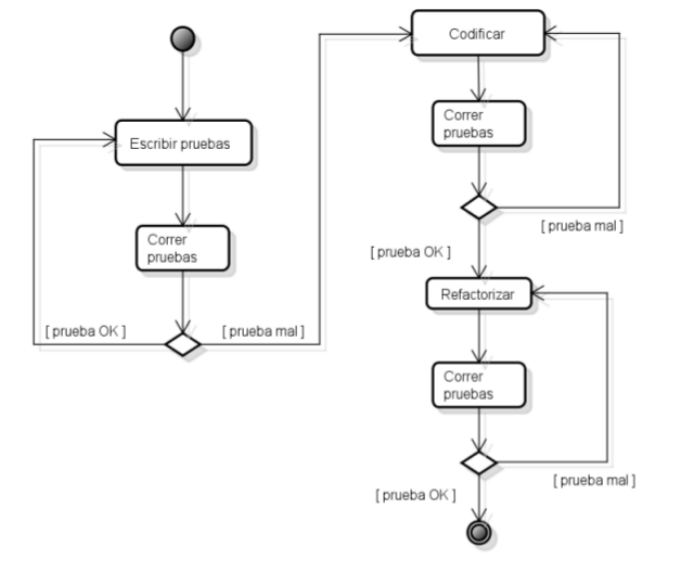
\includegraphics[width=12cm]{./Imagenes/TDD}
    \end{center}
\textbf{}\\
\textbf{}\\
\textbf{}\\
\textbf{3.	Tipos de Test}
\textbf{}\\
\textbf{}\\
\textbf{- Test de aceptación:} es un test que permite comprobar que se está cumpliendo con un requerimiento del negocio. Son pruebas escritas en lenguaje del cliente pero que puede ser ejecutado con la máquina. Esto nos permite probar que el software que estamos desarrollando cumple con las expectativas del cliente y de los usuarios.

\textbf{}\\
\textbf{- Test funcionales:} Si bien, siendo estrictos, todos los tests son funcionales ya que prueban alguna funcionalidad, esta expresión es utilizada para determinar a aquellas pruebas que agrupan a varios tests de aceptación y prueban alguna funcionalidad del negocio propiamente dicha.

\textbf{}\\
\textbf{- Test de sistema:} Integra varias partes del sistema, incluso puede probar toda la aplicación o varias funcionalidades juntas. Estos tests se comportan de manera similar y buscan emular el comportamiento de los usuarios del sistema.

\textbf{}\\
\textbf{- Test unitarios:} Son los tests ineludibles, son los necesarios y los más importantes para los desarrolladores, todo test unitario debe ser rápido, atómico, inocuo e independiente, sino cumple con estas cuatro premisas no es un test unitario.

\end{itemize} 


\end{flushleft}




